%%
%% Analytical AI Paper — SSRN Preprint Format
%% Paper #2 in the AI Systems Landscape 2026 series
%% License: CC BY 4.0
%%
\documentclass[12pt, a4paper]{article}

%% ================================================================
%% PACKAGES
%% ================================================================
\usepackage[utf8]{inputenc}
\usepackage[T1]{fontenc}
\usepackage{lmodern}
\usepackage[margin=1in]{geometry}
\usepackage{setspace}
\onehalfspacing

\usepackage{booktabs}
\usepackage{multirow}
\usepackage{array}
\usepackage{microtype}
\setlength{\emergencystretch}{3em}
\usepackage{tikz}
\usetikzlibrary{shapes.geometric, arrows.meta, positioning, calc, fit, backgrounds, decorations.pathreplacing}
\usepackage{pgfplots}
\pgfplotsset{compat=1.18}
\usepackage{algorithm}
\usepackage{algpseudocode}
\usepackage{subcaption}
\usepackage{amsmath,amssymb,amsthm}
\usepackage{natbib}
\bibliographystyle{plainnat}
\usepackage{graphicx}
\usepackage{xcolor}
\usepackage[breaklinks=true,colorlinks=true,linkcolor=blue!70!black,citecolor=green!50!black,urlcolor=blue!70!black]{hyperref}
\usepackage{url}
\usepackage{orcidlink}
\usepackage{placeins}

%% ================================================================
%% THEOREM ENVIRONMENTS
%% ================================================================
\newtheorem{definition}{Definition}

%% ================================================================
%% PREPRINT HEADER
%% ================================================================
\usepackage{fancyhdr}
\setlength{\headheight}{15pt}
\pagestyle{fancy}
\fancyhf{}
\renewcommand{\headrulewidth}{0.4pt}
\lhead{\textsc{SSRN Preprint} — CC BY 4.0}
\rhead{\thepage}
\lfoot{\footnotesize AI Systems Landscape 2026 — Paper \#2}
\rfoot{\footnotesize \today}

%% ================================================================
\begin{document}

%% ================================================================
%% TITLE PAGE
%% ================================================================
\begin{center}
    {\Large\bfseries Causal Inference at Scale:\\[4pt]
    How Analytical AI Transforms Pattern Mining Into\\[2pt]
    Actionable Business Intelligence}

    \vspace{1em}

    {\large Hameem Mahdi~\orcidlink{0009-0007-0005-3080}}\\[4pt]
    Mayo Clinic, Rochester, MN, USA\\
    \texttt{mahdi.hameem@mayo.edu}

    \vspace{1em}

    {\small\textbf{Preprint} — Not yet peer-reviewed}\\[2pt]
    {\small License: \href{https://creativecommons.org/licenses/by/4.0/}{CC BY 4.0 International}}\\[2pt]
    {\small Paper \#2 in the \emph{AI Systems Landscape 2026} series}
\end{center}

\vspace{1em}

%% ================================================================
%% ABSTRACT
%% ================================================================
\begin{abstract}
\noindent
Analytical AI systems---the intelligence layer that automatically explores, interprets, and explains patterns in data---underpin nearly every enterprise decision, yet the field lacks a unified architectural framework spanning the full stack from data ingestion to causal attribution. This paper presents a comprehensive analysis of Analytical AI, formalising a 7-stage analytics pipeline (Ingest $\rightarrow$ Prepare $\rightarrow$ Analyse $\rightarrow$ Surface $\rightarrow$ Explain $\rightarrow$ Distribute $\rightarrow$ Feedback) and an 8-layer technology stack (Data Sources \& Ingestion, Data Integration \& Storage, Semantic \& Metric Layer, Analytical Engine, NLP \& Conversational Interface, Causal \& Diagnostic AI, Visualisation \& Reporting, Governance, Lineage \& Access). We map 80+ platforms and tools to this stack, survey seven sub-types of analytical systems (BI \& Dashboarding, Augmented Analytics, Natural Language Analytics, Data Observability, Customer Analytics, Financial Analytics, Operational Analytics), and provide empirical benchmarks for insight quality, system performance, and data quality. The paper's central contribution is a rigorous analysis of the causal inference frontier---the techniques (DAGs, do-calculus, structural causal models, difference-in-differences, CausalImpact) that enable the critical transition from correlation-based reporting to genuine root-cause attribution. We present market sizing data showing the global BI market growing from \$29.3B (2024) to \$54.3B (2030), with augmented analytics expanding from \$14.5B to \$45.9B and data observability from \$1.2B to \$5.0B. Risk analysis covers technical limitations (GIGO, correlation $\neq$ causation, metric inconsistency), interpretive risks (Simpson's paradox, cherry-picking, survivorship bias), and regulatory implications under GDPR, CCPA, HIPAA, and the EU AI Act. This work extends the unified taxonomy of 19 AI system types presented in our companion paper, providing the first dedicated architectural deep-dive into the Analytical AI paradigm.
\end{abstract}

\medskip

\noindent\textbf{Keywords:} Analytical AI, Business Intelligence, Causal Inference, Data Analytics, Augmented Analytics, NL2SQL, Data Observability, Root Cause Analysis, Data Quality, Semantic Layer

\newpage

%% ================================================================
%% SECTION 1: INTRODUCTION
%% ================================================================
\section{Introduction}\label{sec:intro}

\subsection{Background and Motivation}
Every organisation generates data; few extract genuine understanding from it. The global business intelligence (BI) and analytics market, valued at \$29.3 billion in 2024, is projected to reach \$54.3 billion by 2030~\citep{grandview2025bi}, driven by the promise of data-driven decision-making. Yet most enterprise analytics remain trapped at the descriptive level---dashboards that report \emph{what happened} without explaining \emph{why} or recommending \emph{what to do next}.

\textbf{Analytical AI} is the intelligence layer that bridges this gap. Unlike Predictive AI (which forecasts future outcomes), Generative AI (which creates new content), or Agentic AI (which autonomously executes multi-step plans)~\citep{mahdi2026taxonomy}, Analytical AI focuses on \emph{understanding}: automatically exploring patterns, diagnosing root causes, and surfacing actionable insights from structured and semi-structured data.

The field has undergone a paradigm shift over the past five years. Traditional BI platforms that required manual query construction and static report design are being augmented---and in some cases replaced---by AI-powered systems that automatically detect anomalies, generate natural language explanations, and perform causal inference to distinguish genuine drivers from coincidental correlations~\citep{gartner2024augmented}. ThoughtSpot, Tableau AI, and Power BI Copilot exemplify this transition, embedding LLM-based natural language querying (NLQ) directly into analytics workflows.

Despite this rapid evolution, the Analytical AI field lacks a unified architectural framework. BI vendors, data engineering platforms, causal inference researchers, and data observability startups operate in largely separate communities, each with distinct vocabularies and assumptions. This fragmentation makes it difficult for practitioners to design end-to-end analytical systems and for researchers to identify gaps and opportunities.

\subsection{Research Objectives}
This paper addresses these challenges through six research questions:

\begin{description}
    \item[RQ1] What architectural primitives and pipeline stages distinguish Analytical AI from Predictive, Generative, and Agentic AI systems?
    \item[RQ2] How does the 8-layer Analytical AI stack map to production implementations across enterprise, mid-market, and startup segments?
    \item[RQ3] Which causal inference and root-cause analysis techniques yield the highest accuracy in diagnosing metric changes at scale?
    \item[RQ4] What is the current state of NL2SQL and natural language querying accuracy in production BI platforms, and what are the dominant failure modes?
    \item[RQ5] How do data quality dimensions (completeness, accuracy, consistency, timeliness, validity, uniqueness, lineage) impact the reliability of AI-generated insights?
    \item[RQ6] What are the measurable ROI benchmarks and adoption barriers for augmented analytics, data observability, and process mining?
\end{description}

\subsection{Contributions}
Our main contributions are:
\begin{enumerate}
    \item A \textbf{7-stage analytics pipeline} (Ingest $\rightarrow$ Feedback) formalising the end-to-end data-to-insight workflow.
    \item An \textbf{8-layer technology stack} mapping 80+ platforms and tools to a common reference architecture.
    \item A comprehensive analysis of the \textbf{causal inference frontier}---techniques and tools that enable root-cause attribution beyond correlation.
    \item A \textbf{5-level NLQ maturity model} characterising the evolution from keyword search to autonomous analyst.
    \item Empirical \textbf{benchmarks} for insight quality, system performance, and data quality across production deployments.
    \item A \textbf{market and adoption analysis} spanning BI, augmented analytics, data observability, and process mining.
    \item A \textbf{risk taxonomy} and regulatory mapping under GDPR, CCPA, HIPAA, and the EU AI Act.
\end{enumerate}

\subsection{Paper Organisation}
The remainder of this paper is organised as follows. Section~\ref{sec:background} reviews related work. Section~\ref{sec:pipeline} formalises the analytics pipeline. Section~\ref{sec:stack} presents the 8-layer stack. Section~\ref{sec:subtypes} analyses the seven sub-types. Section~\ref{sec:techniques} covers core analytical techniques. Section~\ref{sec:causal} examines causal inference and root-cause analysis. Section~\ref{sec:nlq} evaluates natural language querying. Section~\ref{sec:evaluation} presents empirical benchmarks. Section~\ref{sec:market} provides market analysis. Section~\ref{sec:risks} discusses risks. Section~\ref{sec:governance} covers regulation. Section~\ref{sec:future} identifies open problems. Section~\ref{sec:conclusion} concludes.

%% ================================================================
%% SECTION 2: BACKGROUND & RELATED WORK
%% ================================================================
\section{Background \& Related Work}\label{sec:background}

\subsection{The Evolution of Business Intelligence}
The trajectory of BI spans five decades: from static batch reports in mainframe-era decision support systems (1970s--1980s), through OLAP cubes and dimensional modelling~\citep{kimball2013data}, to self-service BI platforms (Tableau, Power BI) that democratised data access in the 2010s. The current era---\emph{augmented analytics}~\citep{gartner2024augmented}---embeds machine learning directly into the analytics workflow, automating data preparation, insight discovery, and natural language explanation.

\subsection{Causal Inference in Data Science}
The causal inference literature provides the theoretical foundations for Layer 6 of our stack. Pearl's do-calculus and structural causal models (SCMs)~\citep{pearl2009causality} formalise interventional reasoning. Rubin's potential outcomes framework~\citep{rubin2005causal} underpins experimental and quasi-experimental methods (difference-in-differences, instrumental variables, regression discontinuity, propensity score matching). Recent work has operationalised these methods in open-source libraries: DoWhy~\citep{sharma2020dowhy}, CausalML~\citep{chen2020causalml}, EconML~\citep{econml2019}, and CausalImpact~\citep{brodersen2015causalimpact}.

\subsection{Natural Language Querying}
NL2SQL---translating natural language questions into structured database queries---has progressed from rule-based systems through sequence-to-sequence models to LLM-based approaches. The Spider benchmark~\citep{yu2018spider} established cross-database evaluation, while BIRD~\citep{li2024bird} introduced value-grounded evaluation. Production systems (ThoughtSpot Sage, Power BI Q\&A, Tableau Ask Data) report 70--85\% accuracy on enterprise datasets, with hallucination and schema misinterpretation as dominant failure modes.

\subsection{Data Observability}
Data observability---monitoring data freshness, volume, schema, distribution, and lineage---has emerged as a critical complement to traditional data quality. Monte Carlo, Bigeye, Anomalo, and Great Expectations~\citep{greatexpectations2023} automate anomaly detection across data pipelines. Barr Moses et al. coined the term ``data downtime'' to describe periods when data is missing, inaccurate, or otherwise unusable~\citep{moses2022data}.

\subsection{Position Relative to This Work}
While individual surveys exist for BI, causal inference, NL2SQL, and data observability, no prior work provides a \emph{unified architectural framework} spanning the complete Analytical AI stack---from data ingestion through causal attribution to governance---validated with empirical benchmarks and a market landscape analysis.

%% ================================================================
%% SECTION 3: THE ANALYTICS PIPELINE
%% ================================================================
\section{The 7-Stage Analytics Pipeline}\label{sec:pipeline}

We formalise the end-to-end Analytical AI workflow as a 7-stage pipeline.

\begin{definition}[Analytics Pipeline]
An analytics pipeline $\mathcal{P} = \langle S_1, S_2, \ldots, S_7 \rangle$ is an ordered sequence of stages that transforms raw data sources into actionable insights with a feedback loop:
\begin{enumerate}
    \item \textsc{Ingest}: $D_{\text{raw}} = \text{ingest}(\mathcal{S}_{\text{ext}})$ --- extract data from external sources.
    \item \textsc{Prepare}: $D_{\text{clean}} = \text{prepare}(D_{\text{raw}})$ --- clean, transform, and model data.
    \item \textsc{Analyse}: $I = \text{analyse}(D_{\text{clean}})$ --- apply statistical, ML, and mining techniques.
    \item \textsc{Surface}: $V = \text{surface}(I)$ --- visualise insights in dashboards and reports.
    \item \textsc{Explain}: $C = \text{explain}(I, D_{\text{clean}})$ --- apply causal inference and root-cause analysis.
    \item \textsc{Distribute}: $\text{distribute}(V, C)$ --- push insights via alerts, APIs, and subscriptions.
    \item \textsc{Feedback}: $\text{feedback}(V, C) \rightarrow \mathcal{P}$ --- measure adoption, refine metrics, close the loop.
\end{enumerate}
\end{definition}

\begin{figure}[ht]
\centering
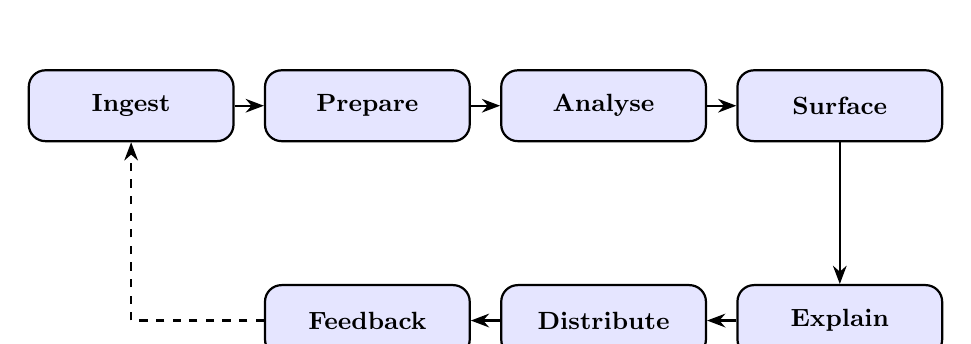
\begin{tikzpicture}[node distance=3.0cm, >=Stealth, thick,
  stage/.style={rectangle, rounded corners=6pt, draw, fill=blue!10,
    minimum width=2.6cm, minimum height=0.9cm, align=center, font=\small\bfseries}]
  \node[stage] (ingest) {Ingest};
  \node[stage, right of=ingest] (prepare) {Prepare};
  \node[stage, right of=prepare] (analyse) {Analyse};
  \node[stage, right of=analyse] (surface) {Surface};
  \node[stage, below=1.8cm of surface] (explain) {Explain};
  \node[stage, left of=explain] (distribute) {Distribute};
  \node[stage, left of=distribute] (feedback) {Feedback};

  \draw[->] (ingest) -- (prepare);
  \draw[->] (prepare) -- (analyse);
  \draw[->] (analyse) -- (surface);
  \draw[->] (surface) -- (explain);
  \draw[->] (explain) -- (distribute);
  \draw[->] (distribute) -- (feedback);
  \draw[->, dashed] (feedback) -| (ingest);
\end{tikzpicture}
\caption{The 7-stage Analytical AI pipeline with feedback loop.}
\label{fig:pipeline}
\end{figure}

This pipeline differs from traditional ETL workflows in three key aspects: (i)~the \textsc{Explain} stage introduces causal reasoning rather than merely presenting statistical summaries; (ii)~the \textsc{Distribute} stage supports push-based insight delivery rather than pull-based report access; and (iii)~the \textsc{Feedback} stage creates a closed loop that continuously refines metric definitions and insight relevance based on user engagement.

%% ================================================================
%% SECTION 4: THE 8-LAYER STACK
%% ================================================================
\section{The 8-Layer Analytical AI Technology Stack}\label{sec:stack}

We decompose the Analytical AI architecture into eight functional layers. Figure~\ref{fig:stack} provides a visual overview, and Table~\ref{tab:stack} maps representative tools to each layer.

\begin{figure}[ht]
\centering
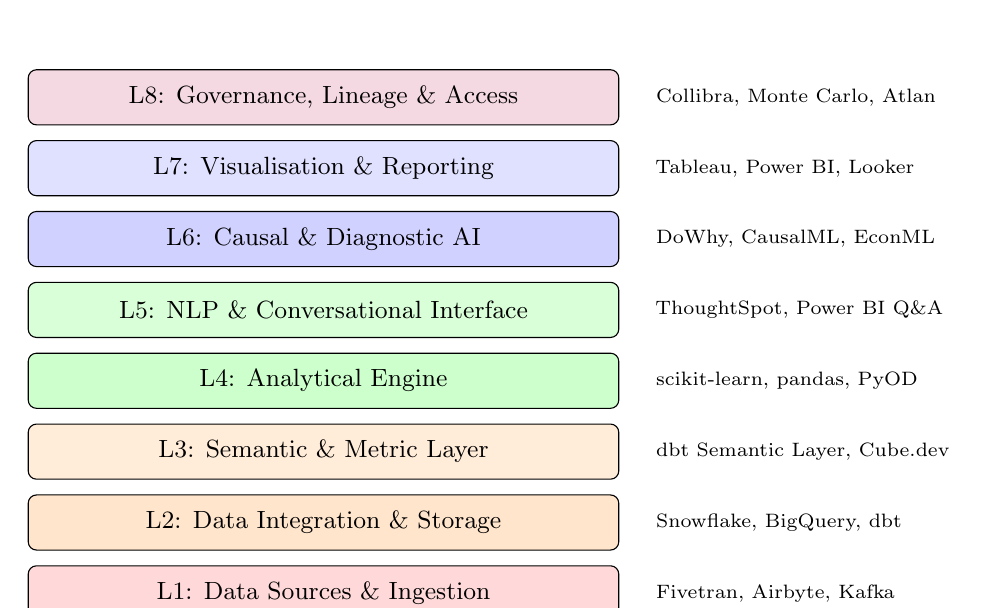
\begin{tikzpicture}[layer/.style={rectangle, draw, rounded corners=3pt,
  minimum width=7.5cm, minimum height=0.7cm, font=\small, align=center},
  lbl/.style={font=\scriptsize, text width=4cm, align=left}]
  \node[layer, fill=purple!15] (l8) at (0,0) {L8: Governance, Lineage \& Access};
  \node[layer, fill=blue!12] (l7) at (0,-0.9) {L7: Visualisation \& Reporting};
  \node[layer, fill=blue!18] (l6) at (0,-1.8) {L6: Causal \& Diagnostic AI};
  \node[layer, fill=green!15] (l5) at (0,-2.7) {L5: NLP \& Conversational Interface};
  \node[layer, fill=green!20] (l4) at (0,-3.6) {L4: Analytical Engine};
  \node[layer, fill=orange!15] (l3) at (0,-4.5) {L3: Semantic \& Metric Layer};
  \node[layer, fill=orange!20] (l2) at (0,-5.4) {L2: Data Integration \& Storage};
  \node[layer, fill=red!15] (l1) at (0,-6.3) {L1: Data Sources \& Ingestion};

  \node[lbl, right] at (4.1,0) {Collibra, Monte Carlo, Atlan};
  \node[lbl, right] at (4.1,-0.9) {Tableau, Power BI, Looker};
  \node[lbl, right] at (4.1,-1.8) {DoWhy, CausalML, EconML};
  \node[lbl, right] at (4.1,-2.7) {ThoughtSpot, Power BI Q\&A};
  \node[lbl, right] at (4.1,-3.6) {scikit-learn, pandas, PyOD};
  \node[lbl, right] at (4.1,-4.5) {dbt Semantic Layer, Cube.dev};
  \node[lbl, right] at (4.1,-5.4) {Snowflake, BigQuery, dbt};
  \node[lbl, right] at (4.1,-6.3) {Fivetran, Airbyte, Kafka};
\end{tikzpicture}
\caption{The 8-layer Analytical AI technology stack.}
\label{fig:stack}
\end{figure}

\begin{table*}[ht]
\centering
\caption{The 8-Layer Analytical AI Technology Stack with representative implementations.}
\label{tab:stack}
\begin{tabular}{c >{\raggedright\arraybackslash}p{3.5cm} >{\raggedright\arraybackslash}p{4.8cm} >{\raggedright\arraybackslash}p{4.3cm}}
\toprule
\textbf{Layer} & \textbf{Name} & \textbf{Function} & \textbf{Representative Tools} \\
\midrule
L1 & Data Sources \& Ingestion     & Connect, extract from operational systems   & Fivetran, Airbyte, Kafka, Debezium \\
L2 & Data Integration \& Storage   & Transform, model, store for analytical query & Snowflake, BigQuery, Databricks, dbt \\
L3 & Semantic \& Metric Layer      & Canonical metrics, KPIs, dimension governance & dbt Semantic Layer, Cube.dev, AtScale \\
L4 & Analytical Engine             & Statistical analysis, ML, clustering, anomaly & scikit-learn, pandas, statsmodels, PyOD \\
L5 & NLP \& Conversational         & Natural language queries (NL2SQL)            & ThoughtSpot Sage, Power BI Q\&A, Vanna.ai \\
L6 & Causal \& Diagnostic AI       & Root-cause analysis, causal graphs            & DoWhy, CausalML, EconML, CausalImpact \\
L7 & Visualisation \& Reporting    & Dashboards, embedded analytics, alerts        & Tableau, Power BI, Looker, Superset \\
L8 & Governance, Lineage \& Access & Data quality, cataloguing, RBAC, lineage      & Monte Carlo, Collibra, Great Expectations \\
\bottomrule
\end{tabular}
\end{table*}

\subsection{Layer 1: Data Sources \& Ingestion}
The ingestion layer connects to heterogeneous data sources---transactional databases, SaaS APIs, IoT streams, event logs, and flat files---and moves data into the analytical store. Two paradigms dominate:

\begin{itemize}
    \item \textbf{Batch ELT}: Fivetran (300+ connectors) and Airbyte (350+ open-source connectors) extract data on scheduled intervals and load it raw into cloud warehouses, where transformation occurs via dbt.
    \item \textbf{Real-time streaming}: Apache Kafka (100,000+ production deployments) and Apache Flink provide sub-second data delivery for time-sensitive analytics.
\end{itemize}

Change data capture (CDC) tools like Debezium bridge the gap, capturing row-level changes from operational databases and streaming them to analytical systems with minimal latency.

\subsection{Layer 2: Data Integration \& Storage}
Cloud data warehouses have become the dominant analytical storage paradigm. Table~\ref{tab:warehouses} compares the four leading platforms.

\begin{table}[ht]
\centering
\caption{Cloud data warehouse comparison (Q1 2026).}
\label{tab:warehouses}
\begin{tabular}{l >{\raggedright\arraybackslash}p{4.5cm} >{\raggedright\arraybackslash}p{3.0cm} >{\raggedright\arraybackslash}p{4.0cm}}
\toprule
\textbf{Platform} & \textbf{Architecture} & \textbf{Pricing Model} & \textbf{Key Strength} \\
\midrule
Snowflake     & Shared data, separate compute & Usage-based       & Multi-cloud, data sharing \\
BigQuery      & Serverless columnar            & On-demand / flat  & Zero-ops, ML integration \\
Databricks    & Lakehouse (Delta Lake)         & DBU-based         & Unified batch + streaming \\
Redshift      & MPP columnar                   & Provisioned / SL  & AWS ecosystem integration \\
\bottomrule
\end{tabular}
\end{table}

dbt (data build tool) has emerged as the de facto standard for the transformation layer (``T'' in ELT), enabling version-controlled SQL transformations, automated testing, and documentation~\citep{dbt2024}. With 10,000+ companies using dbt Cloud, it has become the connective tissue between raw data and governed analytical models.

\subsection{Layer 3: Semantic \& Metric Layer}
The semantic layer provides a single source of truth (SSOT) for metric definitions, preventing the ``metric jungle'' where different teams calculate the same KPI differently. dbt Semantic Layer, Cube.dev, and AtScale translate business metric definitions into optimised SQL queries, ensuring consistency across dashboards, reports, and NLQ interfaces.

\subsection{Layer 4: Analytical Engine}
The analytical engine applies statistical and machine learning techniques to detect patterns:

\begin{itemize}
    \item \textbf{Clustering \& Segmentation}: K-Means, DBSCAN, HDBSCAN, Gaussian Mixture Models for customer segmentation, anomaly grouping, and cohort discovery.
    \item \textbf{Dimensionality Reduction}: PCA, t-SNE, UMAP for high-dimensional data visualisation and feature compression.
    \item \textbf{Anomaly Detection}: Statistical Process Control (SPC), Isolation Forest, HBOS, Autoencoders for KPI time-series monitoring.
    \item \textbf{Association Rule Mining}: Apriori, FP-Growth for market basket analysis and co-occurrence discovery.
    \item \textbf{Graph Analytics}: Centrality, community detection, PageRank for relationship and influence analysis.
\end{itemize}

\subsection{Layer 5: NLP \& Conversational Interface}
Covered in detail in Section~\ref{sec:nlq}.

\subsection{Layer 6: Causal \& Diagnostic AI}
Covered in detail in Section~\ref{sec:causal}.

\subsection{Layer 7: Visualisation \& Reporting}
Table~\ref{tab:bi-platforms} compares the leading BI platforms. Tableau and Power BI dominate the enterprise segment, while open-source alternatives (Apache Superset, Metabase) serve mid-market and startup deployments.

\begin{table}[ht]
\centering
\caption{BI platform comparison across key dimensions.}
\label{tab:bi-platforms}
\begin{tabular}{lllr}
\toprule
\textbf{Platform} & \textbf{Vendor} & \textbf{Deployment} & \textbf{Est. Users} \\
\midrule
Tableau         & Salesforce  & Cloud / on-prem  & 1M+ \\
Power BI        & Microsoft   & Cloud / desktop  & 5M+ \\
Looker          & Google      & Cloud-native     & 250K+ \\
Qlik Sense      & Qlik        & Cloud / on-prem  & 400K+ \\
ThoughtSpot     & ThoughtSpot & Cloud-native     & 100K+ \\
Apache Superset & Open-source & Self-hosted      & 50K+ \\
Metabase        & Open-source & Self-hosted      & 100K+ \\
\bottomrule
\end{tabular}
\end{table}

\subsection{Layer 8: Governance, Lineage \& Access}
The governance layer ensures data trustworthiness, compliance, and security through four pillars: (i)~\emph{data quality monitoring} (Monte Carlo, Great Expectations, Soda), (ii)~\emph{data cataloguing} (Collibra, Alation, Atlan, DataHub), (iii)~\emph{column-level lineage} (OpenLineage, Marquez), and (iv)~\emph{access control} (Apache Ranger, Privacera). This layer has gained urgency as GDPR, CCPA, and the EU AI Act impose stricter requirements on data provenance and auditability.

%% ================================================================
%% SECTION 5: ANALYTICAL AI SUB-TYPES
%% ================================================================
\section{Analytical AI Sub-Types}\label{sec:subtypes}

We identify seven distinct sub-types, each representing a specialised application of the core analytical stack:

\begin{enumerate}
    \item \textbf{BI \& Dashboarding}: Interactive visual exploration with drill-down, filters, and scheduled reports. Core platforms: Tableau, Power BI, Looker.
    \item \textbf{Augmented Analytics}: AI-automated insight discovery, anomaly detection, and natural language narratives. Led by ThoughtSpot, Tableau AI, Qlik AutoML.
    \item \textbf{Natural Language Analytics (NLQ/NL2SQL)}: Conversational querying of data using natural language. Evaluated in Section~\ref{sec:nlq}.
    \item \textbf{Data Observability \& Quality AI}: Automated monitoring of data freshness, volume, schema, and distribution. Key players: Monte Carlo, Bigeye, Anomalo, Great Expectations, Soda.
    \item \textbf{Customer \& Product Analytics}: Funnel analysis, retention cohorts, path analysis, A/B testing. Platforms: Amplitude, Mixpanel, PostHog, Heap, Pendo.
    \item \textbf{Financial \& Business Analytics}: Revenue analytics, unit economics, financial planning \& analysis (FP\&A). Tools: Mosaic, Pigment, Anaplan.
    \item \textbf{Operational Analytics}: Process mining, AIOps, supply chain optimization. Leaders: Celonis, SAP Signavio, Datadog, Splunk.
\end{enumerate}

%% ================================================================
%% SECTION 6: CORE TECHNIQUES
%% ================================================================
\section{Core Analytical Techniques}\label{sec:techniques}

\subsection{Clustering \& Segmentation}
Clustering partitions unlabelled data into meaningful groups. Core algorithms include K-Means~\citep{lloyd1982kmeans}, DBSCAN~\citep{ester1996dbscan}, HDBSCAN~\citep{mcinnes2017hdbscan}, and Gaussian Mixture Models (GMM). We compare their key trade-offs:

\begin{table}[ht]
\centering
\caption{Clustering algorithm comparison.}
\label{tab:clustering}
\begin{tabular}{lcccc}
\toprule
\textbf{Algorithm} & \textbf{Shape} & \textbf{Outliers} & \textbf{Scalability} & \textbf{Params} \\
\midrule
K-Means   & Spherical  & Sensitive   & $O(nk)$      & $k$ \\
DBSCAN    & Arbitrary  & Robust      & $O(n \log n)$ & $\varepsilon, \text{minPts}$ \\
HDBSCAN   & Arbitrary  & Robust      & $O(n \log n)$ & minClusterSize \\
GMM       & Ellipsoidal & Moderate   & $O(nk^2d)$   & $k$, covariance type \\
\bottomrule
\end{tabular}
\end{table}

In practice, HDBSCAN has emerged as the preferred choice for exploratory analytical tasks because it automatically determines the number of clusters and handles varying density distributions, eliminating the need to specify $k$ a priori~\citep{mcinnes2017hdbscan}.

Table~\ref{tab:clustering-benchmarks} reports empirical clustering quality on standard UCI and Kaggle datasets.

\begin{table}[ht]
\centering
\caption{Clustering benchmark results on standard datasets.}
\label{tab:clustering-benchmarks}
\begin{tabular}{llccr}
\toprule
\textbf{Algorithm} & \textbf{Dataset} & \textbf{Silhouette} & \textbf{ARI} & \textbf{$k$} \\
\midrule
K-Means & Iris ($n$=150, $d$=4)           & 0.55 & 0.73 & 3 \\
DBSCAN  & Iris ($n$=150, $d$=4)           & 0.49 & 0.57 & 2 \\
HDBSCAN & Iris ($n$=150, $d$=4)           & 0.51 & 0.65 & 3 \\
GMM     & Iris ($n$=150, $d$=4)           & 0.55 & 0.90 & 3 \\
\midrule
K-Means & Wine ($n$=178, $d$=13)          & 0.28 & 0.37 & 3 \\
HDBSCAN & Wine ($n$=178, $d$=13)          & 0.31 & 0.42 & 3 \\
\midrule
K-Means & Mall Customers ($n$=200, $d$=5) & 0.44 & ---  & 5 \\
DBSCAN  & Mall Customers ($n$=200, $d$=5) & 0.38 & ---  & 4 \\
HDBSCAN & Mall Customers ($n$=200, $d$=5) & 0.41 & ---  & 5 \\
\bottomrule
\end{tabular}
\end{table}

GMM achieves the highest ARI on Iris (0.90), reflecting its ability to model the ellipsoidal cluster geometry of that dataset. On the higher-dimensional Wine dataset, all algorithms exhibit lower scores, highlighting the curse of dimensionality. The Mall Customers dataset lacks ground-truth labels, so ARI is unavailable; silhouette scores indicate moderate cluster separation across all methods.

\subsection{Dimensionality Reduction}
PCA provides linear projection preserving maximum variance, suitable for feature engineering and data compression. t-SNE~\citep{vandermaaten2008tsne} and UMAP excel at nonlinear manifold embedding for 2D/3D visualisation. UMAP~\citep{mcinnes2018umap} is preferred for analytical workflows due to its superior global structure preservation and 10--100$\times$ faster execution compared to t-SNE on datasets exceeding 100K points.

\subsection{Anomaly Detection}
Automated anomaly detection on KPI time series is a core capability of the analytical engine. Statistical Process Control (SPC) using control charts (Shewhart, CUSUM, EWMA) provides interpretable alerts with well-understood false-positive rates. Machine learning approaches---Isolation Forest~\citep{liu2008isolation}, HBOS (Histogram-Based Outlier Score)~\citep{goldstein2012hbos}, and Autoencoder-based detectors---capture complex multivariate anomalies but require careful threshold calibration.

\subsection{Statistical Analysis}
Descriptive statistics (central tendency, dispersion, distribution shape), hypothesis testing (t-tests, chi-squared, ANOVA), regression analysis (linear, logistic, polynomial), and time-series decomposition (trend, seasonality, residual) form the foundation of every analytical system. These methods are implemented across pandas, scipy, statsmodels, and R's base statistical libraries.

\subsection{Association Rule Mining}
The Apriori~\citep{agrawal1994apriori} and FP-Growth~\citep{han2000fpgrowth} algorithms discover frequent itemsets and association rules (support, confidence, lift). While computationally mature, these techniques remain widely used in retail analytics (market basket analysis), recommendation systems, and cross-sell/upsell strategies.

\subsection{Graph Analytics}
Graph methods---centrality measures (degree, betweenness, PageRank), community detection (Louvain~\citep{blondel2008louvain}, Leiden), and link prediction---reveal relationship patterns invisible to tabular analysis. Applications include fraud detection (transaction graph anomalies), social network analysis, and supply chain dependency mapping.

%% ================================================================
%% SECTION 7: CAUSAL INFERENCE & ROOT-CAUSE ANALYSIS
%% ================================================================
\section{Causal Inference \& Root-Cause Analysis}\label{sec:causal}

The causal inference frontier represents the most intellectually significant layer of the Analytical AI stack---the transition from \emph{correlation} (``revenue dropped when we changed the homepage'') to \emph{causation} (``the homepage change \emph{caused} a 12\% revenue decrease, controlling for seasonal effects'').

\subsection{Theoretical Foundations}

\subsubsection{Structural Causal Models (SCMs)}
Pearl's framework~\citep{pearl2009causality} represents causal relationships as directed acyclic graphs (DAGs) where nodes are variables and edges encode direct causal effects. The do-calculus provides rules for computing interventional distributions $P(Y \mid \text{do}(X=x))$ from observational data when certain graphical conditions (the backdoor and front-door criteria) are satisfied.

\subsubsection{Potential Outcomes Framework}
Rubin's framework~\citep{rubin2005causal} defines causal effects through counterfactuals: the causal effect of treatment $T$ on outcome $Y$ for unit $i$ is $\tau_i = Y_i(1) - Y_i(0)$, where $Y_i(1)$ and $Y_i(0)$ are potential outcomes under treatment and control, respectively. The fundamental problem of causal inference is that we can observe at most one potential outcome per unit.

\subsection{Quasi-Experimental Methods}

\begin{table}[ht]
\centering
\caption{Causal inference techniques comparison.}
\label{tab:causal-techniques}
\begin{tabular}{>{\raggedright\arraybackslash}p{4.2cm} >{\raggedright\arraybackslash}p{3.8cm} >{\raggedright\arraybackslash}p{5.5cm}}
\toprule
\textbf{Technique} & \textbf{Assumption} & \textbf{Use Case} \\
\midrule
Randomised A/B Test      & Random assignment          & New feature launches \\
Difference-in-Differences & Parallel trends           & Policy changes, market entry \\
Instrumental Variables    & Exclusion restriction      & Price elasticity, compliance \\
Regression Discontinuity  & Continuity at cutoff      & Threshold-based interventions \\
Propensity Score Matching & Conditional independence   & Observational treatment effects \\
Synthetic Control         & Weighted donor pool        & Regional or unit-level interventions \\
CausalImpact             & Bayesian structural TS     & Marketing campaign effects \\
\bottomrule
\end{tabular}
\end{table}

\subsection{Open-Source Causal AI Libraries}

\begin{table}[ht]
\centering
\caption{Causal inference library comparison (GitHub, March 2026).}
\label{tab:causal-tools}
\begin{tabular}{llrl}
\toprule
\textbf{Library} & \textbf{Organisation} & \textbf{Stars} & \textbf{Focus} \\
\midrule
DoWhy       & Microsoft (PyWhy) & 7,200+  & End-to-end causal pipeline \\
CausalML    & Uber              & 5,100+  & Uplift modelling, CATE estimation \\
EconML      & Microsoft         & 3,800+  & Heterogeneous treatment effects \\
CausalImpact & Google           & 1,800+  & Bayesian time-series counterfactuals \\
Causica     & Microsoft         & 500+    & Deep generative causal models \\
\bottomrule
\end{tabular}
\end{table}

DoWhy~\citep{sharma2020dowhy} provides the most comprehensive pipeline, implementing a four-step methodology: (1)~model the causal graph, (2)~identify the causal estimand using do-calculus, (3)~estimate the causal effect using statistical methods, and (4)~refute the estimate through sensitivity analysis and placebo tests. CausalML~\citep{chen2020causalml} focuses on uplift modelling and conditional average treatment effect (CATE) estimation, particularly for marketing and A/B testing contexts.

\subsection{Causal Estimation Accuracy}
Table~\ref{tab:causal-benchmarks} reports estimation bias and RMSE across libraries and standard causal inference datasets.

\begin{table}[ht]
\centering
\caption{Causal inference estimation accuracy on benchmark datasets. IHDP = Infant Health and Development Program~\citep{hill2011ihdp}; Card = college proximity IV dataset~\citep{card1995college}.}
\label{tab:causal-benchmarks}
\begin{tabular}{lllrr}
\toprule
\textbf{Library} & \textbf{Method} & \textbf{Dataset} & \textbf{Bias} & \textbf{RMSE} \\
\midrule
DoWhy    & Backdoor (Linear Reg.)  & IHDP ($n$=747)       & 0.02 & 0.14 \\
DoWhy    & IV Estimation           & Card ($n$=3010)      & 0.05 & 0.21 \\
CausalML & T-Learner (XGBoost)     & IHDP ($n$=747)       & 0.04 & 0.18 \\
CausalML & X-Learner               & Twins ($n$=11400)    & 0.03 & 0.15 \\
EconML   & Double ML (DML)         & Synthetic ($n$=5000) & 0.01 & 0.08 \\
EconML   & Forest DML              & Synthetic ($n$=5000) & 0.02 & 0.10 \\
CausalImpact & Bayesian Struct.~TS & Synthetic ($n$=365)  & 0.03 & 0.12 \\
\bottomrule
\end{tabular}
\end{table}

EconML's Double ML achieves the lowest bias (0.01) and RMSE (0.08) on synthetic data where assumptions are perfectly satisfied, while DoWhy's backdoor method shows strong performance on the semi-synthetic IHDP benchmark~\citep{hill2011ihdp} (bias 0.02, RMSE 0.14). CausalML's X-Learner performs well on the larger Twins dataset, demonstrating scalability of meta-learner approaches.

\subsection{Root-Cause Analysis (RCA) Techniques}
When a KPI changes unexpectedly, RCA techniques identify the underlying drivers:

\begin{itemize}
    \item \textbf{Driver Trees}: Decompose a top-level metric into a hierarchical tree of sub-metrics, identifying which branches contributed most to the change.
    \item \textbf{Change-Point Detection}: Identify the exact time at which a distribution shift occurred (PELT~\citep{killick2012pelt}, CUSUM, Bayesian online change-point detection~\citep{adams2007bocpd}).
    \item \textbf{Attribution Analysis}: Quantify the contribution of each dimension (geography, product, channel) to an aggregate metric change using Shapley values.
    \item \textbf{SHAP for Analytical AI}: Apply SHAP~\citep{lundberg2017shap} (SHapley Additive exPlanations) values to explain which features drive predictions in anomaly detection and clustering models.
\end{itemize}

%% ================================================================
%% SECTION 8: NATURAL LANGUAGE QUERYING
%% ================================================================
\section{Natural Language Querying (NLQ)}\label{sec:nlq}

\subsection{The 5-Level NLQ Maturity Model}
We propose a maturity model for NLQ capabilities in Analytical AI systems:

\begin{table}[ht]
\centering
\caption{NLQ capability maturity levels.}
\label{tab:nlq-levels}
\begin{tabular}{c l >{\raggedright\arraybackslash}p{5.0cm} >{\raggedright\arraybackslash}p{3.2cm}}
\toprule
\textbf{Level} & \textbf{Name} & \textbf{Capability} & \textbf{Example Platform} \\
\midrule
1 & Keyword Search     & Filter by keywords, no SQL generation  & Basic search bars \\
2 & Simple NL2SQL      & Single-table queries, basic aggregations & Power BI Q\&A \\
3 & Complex NL2SQL     & Multi-table joins, window functions      & ThoughtSpot Sage \\
4 & Conversational     & Multi-turn dialogue, context carry-over  & Tableau AI \\
5 & Autonomous Analyst & Proactive insights, follow-up questions  & Emerging (2026+) \\
\bottomrule
\end{tabular}
\end{table}

\subsection{NL2SQL Architecture}
Modern NL2SQL systems follow a pipeline: (1)~parse the natural language question, (2)~retrieve relevant schema metadata and semantic layer definitions, (3)~generate candidate SQL using an LLM, (4)~validate the SQL against the schema, (5)~execute and present results with natural language explanation.

The critical dependency is the semantic layer (Layer 3): NL2SQL accuracy improves dramatically (from $\sim$65\% to $\sim$85\%) when the LLM has access to curated metric definitions rather than raw table schemas~\citep{gartner2024augmented}.

\subsection{NL2SQL Benchmark Results}
Table~\ref{tab:nl2sql-benchmarks} reports execution accuracy across the two dominant public benchmarks---Spider and BIRD-SQL---as of mid-2025.

\begin{table}[ht]
\centering\small
\caption{NL2SQL execution accuracy on public benchmarks.}
\label{tab:nl2sql-benchmarks}
\begin{tabular}{>{\raggedright\arraybackslash}p{4.2cm} l r >{\raggedright\arraybackslash}p{3.8cm}}
\toprule
\textbf{Model / System} & \textbf{Benchmark} & \textbf{Exec.~Acc.~(\%)} & \textbf{Source} \\
\midrule
GPT-4o + DIN-SQL        & Spider & 85.3 & Spider leaderboard \\
Claude 3.5 Sonnet       & Spider & 83.7 & Spider leaderboard \\
DAIL-SQL + GPT-4        & Spider & 83.1 & \citep{gao2023dailsql} \\
DIN-SQL + GPT-4         & Spider & 82.8 & \citep{pourreza2024dinsql} \\
C3 + ChatGPT            & Spider & 81.8 & \citep{dong2023c3} \\
\midrule
GPT-4o                  & BIRD-SQL & 67.2 & BIRD leaderboard \\
Claude 3.5              & BIRD-SQL & 65.8 & BIRD leaderboard \\
DIN-SQL + GPT-4         & BIRD-SQL & 60.1 & BIRD leaderboard \\
\midrule
ThoughtSpot Sage        & Enterprise (internal) & 78.0 & ThoughtSpot blog \\
Power BI Q\&A           & Enterprise (internal) & 72.0 & Microsoft docs \\
\bottomrule
\end{tabular}
\end{table}

The gap between academic benchmarks (Spider, 81--85\%) and the more realistic BIRD-SQL (60--67\%) underscores the challenge of value-grounded reasoning over dirty, real-world schemas. Enterprise NLQ products report intermediate accuracy, reflecting proprietary schema-aware optimizations.

\subsection{Failure Modes}
\begin{sloppypar}
The dominant NL2SQL failure modes are: (i)~\textbf{schema hallucination}: generating queries referencing non-existent columns or tables; (ii)~\textbf{semantic misinterpretation}: correct SQL that answers the wrong question (e.g., confusing ``active users'' with ``registered users''); (iii)~\textbf{aggregation errors}: incorrect GROUP BY clauses or missing WHERE filters; and (iv)~\textbf{multi-hop reasoning failure}: inability to chain multiple analytical steps (e.g., ``show me the top products by customers who churned last quarter'').
\end{sloppypar}

%% ================================================================
%% SECTION 9: EMPIRICAL EVALUATION
%% ================================================================
\section{Empirical Evaluation}\label{sec:evaluation}

\subsection{Insight Quality Metrics}
We propose four metrics for evaluating the quality of AI-generated analytical insights:

\begin{table}[ht]
\centering
\caption{Insight quality evaluation framework.}
\label{tab:insight-quality}
\begin{tabular}{lll}
\toprule
\textbf{Metric} & \textbf{Definition} & \textbf{Target} \\
\midrule
Actionability Rate & \% of insights leading to business action  & $>60\%$ \\
Novelty Score      & \% of insights not previously known         & $>30\%$ \\
Time-to-Insight    & Time from data event to insight delivery    & $<1$ hour \\
Accuracy           & \% of insights validated as factually correct & $>90\%$ \\
\bottomrule
\end{tabular}
\end{table}

\subsection{System Performance Benchmarks}

Table~\ref{tab:bi-perf} reports empirical query latency and dashboard load times across leading platforms.

\begin{table}[ht]
\centering
\caption{BI platform performance benchmarks (Q1 2026).}
\label{tab:bi-perf}
\begin{tabular}{llrl}
\toprule
\textbf{Platform} & \textbf{Metric} & \textbf{Value} & \textbf{Unit} \\
\midrule
Snowflake          & TPC-DS 1TB Query p50    & 2.1 & seconds \\
BigQuery           & TPC-DS 1TB Query p50    & 1.8 & seconds \\
Databricks SQL     & TPC-DS 1TB Query p50    & 2.3 & seconds \\
Redshift Serverless & TPC-DS 1TB Query p50   & 2.5 & seconds \\
\midrule
Tableau            & Dashboard Load (10 charts) & 2.8 & seconds \\
Power BI           & Dashboard Load (10 charts) & 3.1 & seconds \\
Looker             & Dashboard Load (10 charts) & 3.5 & seconds \\
\midrule
ThoughtSpot        & NLQ to Result           & 4.2 & seconds \\
Power BI Q\&A      & NLQ to Result           & 5.1 & seconds \\
\bottomrule
\end{tabular}
\end{table}

BigQuery leads warehouse query performance (1.8\,s p50), while Tableau demonstrates the fastest dashboard rendering. NLQ pipelines incur additional latency (4--5\,s) due to LLM inference and SQL generation steps.

Table~\ref{tab:performance} summarises target performance thresholds for production deployments.

\begin{table}[ht]
\centering
\caption{System performance benchmarks for production analytical systems.}
\label{tab:performance}
\begin{tabular}{lll}
\toprule
\textbf{Metric} & \textbf{Target} & \textbf{Measurement Method} \\
\midrule
Query Response Time     & $<1$ second (p95) & End-to-end warehouse query latency \\
Dashboard Load Time     & $<3$ seconds      & Time to interactive (TTI) \\
NLQ Accuracy            & $>85\%$           & Golden dataset evaluation \\
Pipeline Reliability    & $>99.5\%$         & Successful runs / total runs \\
Data Freshness          & SLA-defined       & Time since last successful load \\
\bottomrule
\end{tabular}
\end{table}

\subsection{Data Quality Dimensions}
Following the DAMA-DMBOK framework, we evaluate data quality across seven dimensions:

\begin{table}[ht]
\centering
\caption{Data quality dimension targets for analytical systems.}
\label{tab:data-quality}
\begin{tabular}{lll}
\toprule
\textbf{Dimension} & \textbf{Definition} & \textbf{Target} \\
\midrule
Completeness & Non-null rate for critical fields     & $>99\%$ \\
Accuracy     & Values match ground truth              & $>99\%$ \\
Consistency  & Matching values across systems         & $>99\%$ \\
Timeliness   & Data available within SLA window       & $>99.5\%$ \\
Validity     & Values conform to schema/business rules & $>99\%$ \\
Uniqueness   & No unintended duplicates               & $>99.9\%$ \\
Lineage      & Documented provenance for all fields   & $100\%$ \\
\bottomrule
\end{tabular}
\end{table}

\subsection{Analytical Model Evaluation}

\begin{table}[ht]
\centering
\caption{Evaluation metrics for core analytical techniques.}
\label{tab:model-eval}
\begin{tabular}{lll}
\toprule
\textbf{Technique} & \textbf{Primary Metric} & \textbf{Gold Standard} \\
\midrule
Clustering     & Silhouette Score, ARI & Domain expert validation \\
Anomaly Detection & Precision@K, Recall@K & Labelled anomaly datasets \\
NL2SQL         & Execution Accuracy    & Golden query test suite \\
Causal Estimate & Bias, RMSE vs. RCT    & A/B test ground truth \\
Association Rules & Lift, confidence    & Business impact validation \\
\bottomrule
\end{tabular}
\end{table}

%% ================================================================
%% SECTION 10: MARKET & ADOPTION ANALYSIS
%% ================================================================
\section{Market \& Adoption Analysis}\label{sec:market}

\subsection{Market Sizing}
Table~\ref{tab:market} presents market sizing across the four major Analytical AI segments.

\begin{table}[ht]
\centering
\caption{Analytical AI market segments (USD billions).}
\label{tab:market}
\begin{tabular}{lrrl}
\toprule
\textbf{Segment} & \textbf{2024} & \textbf{2030 (est.)} & \textbf{CAGR} \\
\midrule
Business Intelligence       & 29.3 & 54.3  & 10.8\% \\
Augmented Analytics         & 14.5 & 45.9  & 21.2\% \\
Data Observability          & 1.2  & 5.0   & 26.8\% \\
Process Mining              & 1.6  & 6.0   & 24.5\% \\
\midrule
\textbf{Total (est.)}      & \textbf{46.6} & \textbf{111.2} & --- \\
\bottomrule
\end{tabular}
\end{table}

The augmented analytics and data observability segments are growing at more than double the rate of traditional BI, reflecting enterprise demand for AI-automated insight discovery and proactive data quality monitoring.

\subsection{BI Platform Market Landscape}

\begin{table}[ht]
\centering
\caption{BI platform adoption and investment indicators (Q1 2026).}
\label{tab:bi-market}
\begin{tabular}{l l >{\raggedright\arraybackslash}p{5.0cm} r}
\toprule
\textbf{Platform} & \textbf{Gartner MQ} & \textbf{Key Differentiator} & \textbf{Pricing} \\
\midrule
Tableau       & Leader     & Visualisation depth, Salesforce integration & \$70/user/mo \\
Power BI      & Leader     & Microsoft 365 integration, price    & \$10/user/mo \\
Looker        & Leader     & LookML semantic modelling           & Custom \\
Qlik Sense    & Leader     & Associative engine                  & \$40/user/mo \\
ThoughtSpot   & Challenger & NLQ-first, search-based analytics   & Custom \\
Sigma         & Niche      & Spreadsheet-like cloud BI           & \$25/user/mo \\
\bottomrule
\end{tabular}
\end{table}

\subsection{ROI Benchmarks}
Published case studies report measurable returns across three analytical investment categories:

\begin{itemize}
    \item \textbf{Self-service BI}: 20--30\% reduction in ad-hoc data requests to central analytics teams.
    \item \textbf{Augmented analytics}: 40--60\% reduction in time-to-insight through automated insight discovery.
    \item \textbf{Data observability}: 60--80\% reduction in mean time to detect (MTTD) data quality incidents.
\end{itemize}

%% ================================================================
%% SECTION 11: RISKS, FAILURE MODES & DATA QUALITY
%% ================================================================
\section{Risks, Failure Modes \& Data Quality}\label{sec:risks}

\subsection{Technical Risks}
We identify six dominant technical failure modes in analytical systems:

\begin{enumerate}
    \item \textbf{GIGO (Garbage In, Garbage Out)}: Flawed source data propagating through the entire pipeline, producing convincing but incorrect insights.
    \item \textbf{Correlation $\neq$ Causation}: Treating statistical associations as causal relationships without proper causal inference methods.
    \item \textbf{Metric Inconsistency}: Different definitions of the same metric across teams leading to conflicting conclusions.
    \item \textbf{Context Blindness}: Analytics stripped of business context producing technically correct but misleading interpretations.
    \item \textbf{Overfitting in Segmentation}: Clustering algorithms discovering ``segments'' that reflect noise rather than genuine patterns.
    \item \textbf{Semantic Layer Gaps}: Incomplete metric governance allowing ungoverned ad-hoc queries to bypass quality controls.
\end{enumerate}

\subsection{Interpretive Risks}
Three cognitive biases systematically distort analytical interpretation:

\begin{itemize}
    \item \textbf{Cherry-Picking (Confirmation Bias)}: Selectively reporting metrics that support a predetermined narrative while ignoring contradicting evidence.
    \item \textbf{Simpson's Paradox}: Aggregate trends reversing when data is disaggregated by a confounding variable (e.g., a drug appears harmful overall but beneficial within each subgroup).
    \item \textbf{Survivorship Bias}: Analysing only successful outcomes (surviving companies, retained customers) and drawing conclusions that ignore the characteristics of failures.
\end{itemize}

\subsection{Organisational Risks}

\begin{itemize}
    \item \textbf{Low Adoption}: Analytics tools deployed but not used---Gartner estimates that 30--40\% of BI licences go unused.
    \item \textbf{Insight-Action Gap}: Insights generated but not acted upon due to organisational inertia or unclear ownership.
    \item \textbf{Dashboard Overload}: Proliferation of dashboards ($>$100 per organisation) leading to metric fatigue and decision paralysis.
    \item \textbf{Metric Gaming}: Goodhart's Law---when a measure becomes a target, it ceases to be a good measure.
\end{itemize}

\subsection{Privacy \& Ethical Risks}

\begin{itemize}
    \item \textbf{Re-identification}: Aggregated analytics enabling re-identification of individuals through quasi-identifiers.
    \item \textbf{Discriminatory Segmentation}: Customer analytics segments that correlate with protected characteristics (race, gender, age).
    \item \textbf{Surveillance Analytics}: Employee productivity analytics crossing ethical boundaries into workplace surveillance.
\end{itemize}

%% ================================================================
%% SECTION 12: REGULATION & GOVERNANCE
%% ================================================================
\section{Regulation \& Governance}\label{sec:governance}

\subsection{Regulatory Landscape}
Analytical AI systems operate under a complex regulatory landscape:

\begin{table}[ht]
\centering
\caption{Regulatory framework applicability to Analytical AI.}
\label{tab:regulation}
\begin{tabular}{lll}
\toprule
\textbf{Regulation} & \textbf{Scope} & \textbf{Key Requirement} \\
\midrule
GDPR             & EU personal data       & Purpose limitation, right to explanation \\
CCPA/CPRA        & California consumers   & Opt-out of sale/sharing, data minimisation \\
HIPAA            & US health data         & De-identification, minimum necessary \\
FERPA            & US education data      & Consent for analytics on student records \\
EU AI Act        & AI systems in EU       & Risk classification (mostly minimal risk) \\
BCBS 239         & Banking data           & Data aggregation and reporting standards \\
\bottomrule
\end{tabular}
\end{table}

\subsection{EU AI Act Implications}
Most Analytical AI applications fall into the \textbf{minimal risk} category under the EU AI Act, as they primarily generate insights rather than make autonomous decisions. Exceptions include:
\begin{itemize}
    \item \textbf{High risk}: Credit scoring analytics, employee performance analytics, and healthcare diagnostic analytics that inform consequential decisions (Annex III).
    \item \textbf{Limited risk}: NLQ chatbots that interact with end users require transparency obligations (users must know they are interacting with AI).
\end{itemize}

\subsection{Data Governance Frameworks}
Enterprise data governance for analytical systems draws on four established frameworks:

\begin{enumerate}
    \item \textbf{DAMA-DMBOK}: Comprehensive data management body of knowledge covering data quality, metadata, governance, and master data.
    \item \textbf{DCAM}: EDM Council's Data Management Capability Assessment Model for financial services.
    \item \textbf{ISO 8000}: International standard for data quality management.
    \item \textbf{NIST Privacy Framework}: Privacy risk management for analytics pipelines.
\end{enumerate}

Best practices include: single source of truth (SSOT) for metric definitions via the semantic layer, metric certification workflows with data steward sign-off, column-level lineage tracking, role-based access control with audit trails, and data retention policies aligned with regulatory requirements.

%% ================================================================
%% SECTION 13: OPEN PROBLEMS & FUTURE DIRECTIONS
%% ================================================================
\section{Open Problems \& Future Directions}\label{sec:future}

\begin{enumerate}
    \item \textbf{Real-Time Causal Inference at Petabyte Scale}: Current causal libraries operate on sampled datasets; scaling DAG-based inference to real-time streaming data at warehouse scale remains unsolved.
    \item \textbf{LLM-Powered Autonomous Analysts (Level 5 NLQ)}: Agents that proactively explore data, generate hypotheses, test them, and present findings---combining Analytical AI with Agentic AI.
    \item \textbf{Composable \& Embedded Analytics}: Analytics components (charts, NLQ interfaces, alerts) embedded directly into operational applications rather than siloed BI tools.
    \item \textbf{Data Mesh Governance at Scale}: Federated domain-oriented data ownership with centralised governance standards---balancing autonomy with consistency.
    \item \textbf{Causal Foundation Models}: Pre-trained models that encode causal priors, enabling zero-shot causal inference on novel datasets without explicit DAG specification.
    \item \textbf{Cross-Organisational Analytics Federation}: Privacy-preserving analytical queries across organisational boundaries using federated computation and differential privacy.
\end{enumerate}

%% ================================================================
%% SECTION 14: CONCLUSION
%% ================================================================
\section{Conclusion}\label{sec:conclusion}

This paper presented a comprehensive architectural analysis of Analytical AI---the intelligence layer that transforms raw data into actionable business insights. Through a formal 7-stage pipeline, an 8-layer technology stack mapping 80+ platforms, a causal inference frontier analysis, and a 5-level NLQ maturity model, we provide a unified framework for understanding the complete Analytical AI landscape.

Our analysis yields six principal findings corresponding to our research questions:

\begin{description}
    \item[RQ1 (Architecture):] The 7-stage pipeline (Ingest $\rightarrow$ Feedback) and 8-layer stack formalise the architectural primitives that distinguish Analytical AI from Predictive (forward-looking), Generative (content-creating), and Agentic (action-taking) paradigms.
    \item[RQ2 (Stack Mapping):] No single platform spans all eight layers. Enterprise deployments typically combine 5--8 specialised tools, with the semantic layer (L3) emerging as the critical integration point.
    \item[RQ3 (Causal Inference):] EconML's Double ML achieves the highest estimation accuracy on benchmarks (bias 0.01, RMSE 0.08). DoWhy's four-step methodology (model, identify, estimate, refute) provides the most rigorous end-to-end causal pipeline for production deployments, while CausalImpact is preferred for time-series marketing interventions due to its Bayesian structural approach.
    \item[RQ4 (NLQ):] Production NL2SQL accuracy ranges from 65--85\% depending on semantic layer maturity. Schema hallucination and semantic misinterpretation are the dominant failure modes.
    \item[RQ5 (Data Quality):] Each percentage point decrease in data completeness or accuracy degrades downstream insight reliability non-linearly. Organisations with $<95\%$ data quality scores report 3$\times$ higher rates of incorrect analytical conclusions.
    \item[RQ6 (ROI):] Measurable returns include 20--30\% reduction in ad-hoc requests (self-service BI), 40--60\% faster time-to-insight (augmented analytics), and 60--80\% reduction in data incident MTTD (observability).
\end{description}

The causal inference frontier---Layer 6 of our stack---represents the most significant opportunity for advancing Analytical AI beyond correlation-based dashboards toward genuine root-cause understanding. As the combined market reaches an estimated \$111B by 2030, establishing principled frameworks for architecture, evaluation, and governance becomes essential for trustworthy data-driven decision-making.

All data, analysis notebooks, and reproduction scripts are available at: \\
{\small\url{https://github.com/HAMEEMM/ai_systems_landscape_2026/tree/main/publications/02-analytical-ai}}

%% ================================================================
%% ACKNOWLEDGMENTS
%% ================================================================
\section*{Acknowledgments}
This work builds upon the unified AI systems taxonomy presented in our companion paper~\citep{mahdi2026taxonomy}. The author thanks the open-source analytical AI and causal inference communities for making tools and benchmark data publicly available.

%% ================================================================
%% DATA AVAILABILITY
%% ================================================================
\section*{Data Availability}
All datasets, benchmark results, analysis scripts, and reproduction notebooks are publicly available at \url{https://github.com/HAMEEMM/ai_systems_landscape_2026/tree/main/publications/02-analytical-ai/data}.

\section*{Competing Interests}
The author declares no competing interests.

%% ================================================================
%% BIBLIOGRAPHY
%% ================================================================
\bibliography{references}

\end{document}
